%Section Comments: "Second generation intact stability criteria" seems more commonly used. It would help to specify a specific time period instead of saying "a long time."
\section{Summary of Paper \ref{pap:rolldamping}}
\subsection*{"\nameref{pap:rolldamping}"}
System identification of ship roll motion, which includes roll damping and stiffness, is developed in Paper \ref{pap:rolldamping}. Parametric roll was observed by \textcite{froude_rolling_1861} and has been a focus of the marine research community since the early 1950s \parencite{galeazzi_early_2013}; it has received even more attention since \textcite{france_investigation_2001} demonstrated that the APL China casualty in 1998, where a post-Panamax C11 class container ship lost almost a third of its containers, was most likely caused by head sea parametric rolling. The damping of roll motion plays an important role in these phenomena. Previous literature demonstrates that the relatively small difference in the roll damping prediction obtained with small method variation may contribute to the difference between severe roll angles and much less noticeable motions \cite{soder_ikeda_2019}.

The objective of Paper \ref{pap:rolldamping} was to improve the roll damping predictions for modern ships. The roll damping was studied using time series data from 250 (see \autoref{fig:ship_types}) roll decay tests (see \autoref{sec:roll}) assembled by the Maritime Dynamics Laboratory at SSPA Sweden AB (\href{www.sspa.se}{www.sspa.se}). The work was divided into the following sub tasks (also summarized in \autoref{fig:paper1_overview}): 
\vspace{5pt}
\begin{itemize}
    \setlength\itemsep{5pt}
    \item Find the mathematical model that is the best representation of the roll motion.
    \item Identify the parameters in this model for all the tests.
    \item Compare the identified parameters with state of art predictions.
    \item Develop a generic roll damping model for all ships using the identified parameters.
    \begin{itemize}
        \item Grey-box model
        \item Black-box model
    \end{itemize}
\end{itemize}
\vspace{5pt}
\begin{figure}[!htb]
    \centering
    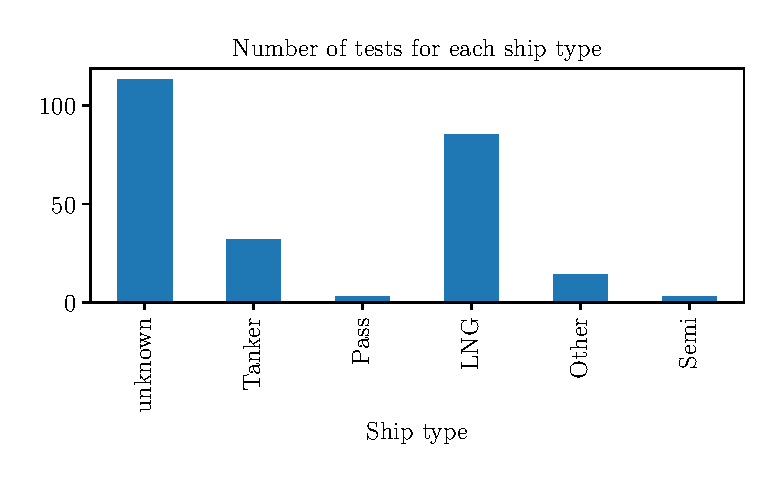
\includegraphics[width=0.6\columnwidth]{kappa/images/ship_types.eps}
    \caption{Number of tests per ship type.}
    \label{fig:ship_types}
\end{figure}
\begin{figure}[!htb]
    \centering
\begin{tikzpicture}[node distance=3cm]
\node (data_collection) at (0,0) {Data collection:};
\node (roll_decay_DB) [database,label=below:Roll decay DB, right of=data_collection, xshift=-0.5cm]{};
\node (PIT) [process, right of=roll_decay_DB, xshift=0.5cm] {PIT};
\node (damping_DB) [database, label=below:Damping DB, right of=PIT, xshift=0cm] {};
\path (roll_decay_DB) -- node(time_series)[xshift=3.0cm]{Time series} -- (PIT);
\draw [arrow] (roll_decay_DB) -- (time_series) -- (PIT);
\path (PIT) -- node(B){B} (damping_DB);
\draw [arrow] (PIT) -- (B) -- (damping_DB);

\node (comparison)[below of=data_collection, yshift=0.5cm]{Comparison:};
%plot:
\node (origo)[right of=comparison, xshift=-0.5cm, yshift=-1cm];
\node(y)[above of=origo, yshift=-1cm]{Simplified ikeda};
\node(x)[right of=origo, xshift=-1cm]{Damping DB};
\draw[->](origo) -- (y);
\draw[->](origo) -- (x);
\draw node[anchor=south, right of=origo, xshift=-3cm, yshift=0cm] {\textbullet};
\draw node[anchor=south, right of=origo, xshift=-2.5cm, yshift=0.6cm] {\textbullet};
\draw node[anchor=south, right of=origo, xshift=-2cm, yshift=1cm] {\textbullet};
\draw node[anchor=south, right of=origo, xshift=-2cm, yshift=1.2cm] {\textbullet};
\draw node[anchor=south, right of=origo, xshift=-1.5cm, yshift=1.7cm] {\textbullet};
\draw node[anchor=south, right of=origo, xshift=-1.5cm, yshift=1.3cm] {\textbullet};
\draw node[anchor=south, right of=origo, xshift=-1cm, yshift=2cm] {\textbullet};

\node (regressions)[below of=comparison, yshift=-0.5cm]{Regressions:};
\node (damping_DB2) [database,label=below:Damping DB, right of=regressions, xshift=-0.5cm]{};
\node (grey_box) [grey-box, right of=damping_DB2, xshift=0.5cm, yshift=1.5cm] {Grey-box};
\node (black_box) [black-box, below of=grey_box, yshift=1.5cm] {Black-box};
\draw [arrow] (damping_DB2) |- (grey_box);
\draw [arrow] (damping_DB2) -- (black_box);
\end{tikzpicture}
    \caption{Overview of the work conducted for Paper \ref{pap:rolldamping}.}
    \label{fig:paper1_overview}
\end{figure}
System identification on the time series from the roll decay database was performed with the linear (\autoref{eq:roll_decay_equation_himeno_linear}), quadratic (\autoref{eq:roll_decay_equation_himeno_quadratic_b}), and cubic models (\autoref{eq:roll_decay_equation_cubic}). Estimated roll damping parameters were used to build a roll damping database. The database could be compared to corresponding predictions with the simplified Ikeda's method \cite{kawahara_simple_2011}, which is the state of art prediction for ship roll damping.
The generic roll damping model was developed as a grey-box model and a black-box model.
\subsection{Best mathematical model for the roll motion}
System identification on the linear, quadratic, and cubic models was conducted using both the ``integration approach'' (\autoref{sec:integration_approach}) and the ``derivation approach'' (\autoref{sec:derivation_approach}) where the best parameter estimations were obtained using the ``integration approach''.
Results from the simulations with the identified models (from one of the roll-decay tests) are presented in \autoref{fig:roll_decay_compare}. The cubic and quadratic models reproduce the model test well, and the linear model is too simple to provide an accurate representation for both smaller and larger roll angles. The amplitude decrement $\phi_a$ and roll damping $B$ for each oscillation can be visualized, as seen in \autoref{fig:roll_decay}.
\begin{figure}[h!]
    \centering
    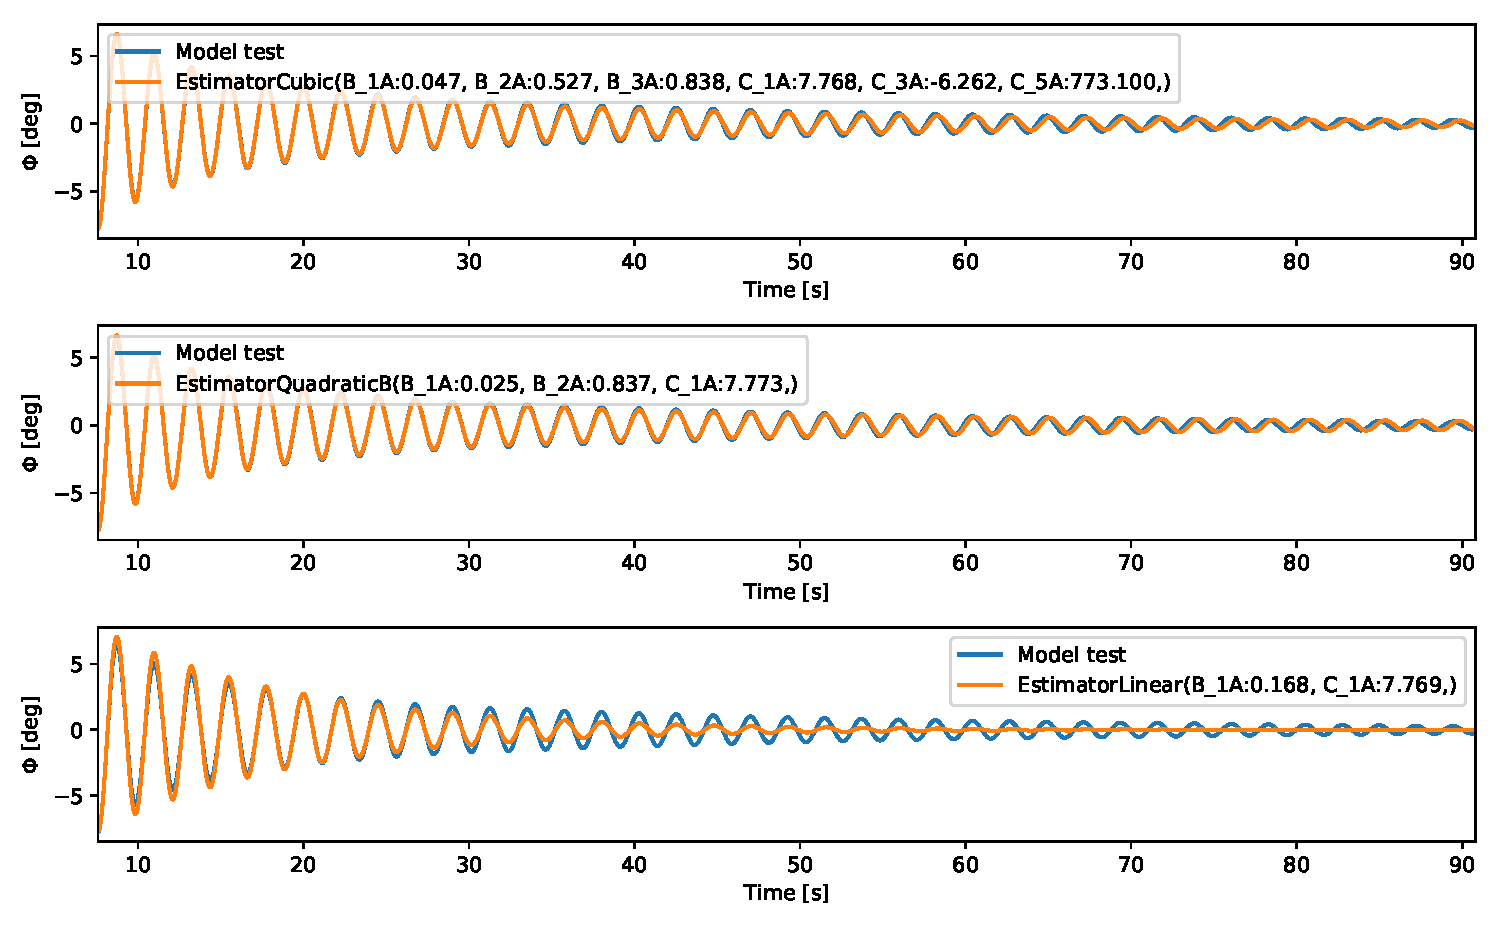
\includegraphics[width=\linewidth]{kappa/images/roll_decay_model_compare.pdf}
    \caption{Roll decay estimation with identified cubic, quadratic, and linear models.}
    \label{fig:roll_decay_compare}
\end{figure}
\begin{figure}[h!]
    \begin{subfigure}[b]{0.45\textwidth}
        \centering
        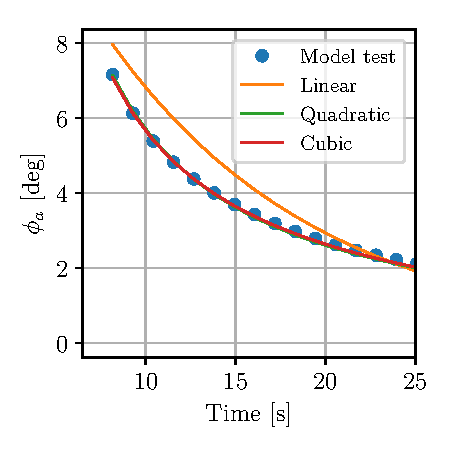
\includegraphics[width=0.9\linewidth]{kappa/images/roll_decay_amplitude.pdf}
        \caption{Amplitude decrements.}
        \label{fig:roll_decay_amplitude}
    \end{subfigure}
        ~ %add desired spacing between images, e. g. ~, \quad, \qquad, \hfill etc. 
      %(or a blank line to force the subfigure onto a new line)
    \begin{subfigure}[b]{0.45\textwidth}
        \centering
        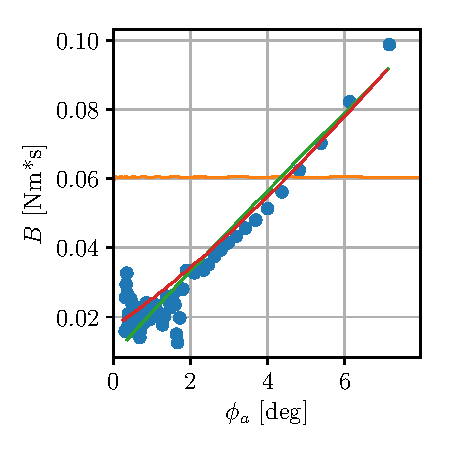
\includegraphics[width=0.9\linewidth]{kappa/images//roll_decay_damping.pdf}
        \caption{Dampings.}
        \label{fig:roll_decay_damping}
    \end{subfigure}
    \caption{Roll decay model test, linear-, quadratic- and cubic-model.}
    \label{fig:roll_decay}
\end{figure}
The goodness of fit for the linear, quadratic, and cubic models can be expressed using the coefficient of determination:
\begin{equation} \label{eq:R2}
%R^2=1-\frac{SS_{res}}{SS_{tot}}
R^2=1-\frac{\sum\limit_{i=1}^{n}(\phi_{i}-\hat{\phi}_i)^2}{\sum\limit_{i=1}^{n}(\phi_i-\bar \phi)^2}
\end{equation}
where $\phi_i$ is the model test roll angle at time step $i$, $\bar \phi$ is the mean roll angle from the model test, and $\hat{\phi}_i$ is the predicted roll angle (with the linear, quadratic, or cubic model). The average goodness of fit $R^2$ was 0.995 for the cubic model, 0.993 for the quadratic model, and 0.986 for the linear model. These values indicate that the quadratic model is almost as useful as the cubic model for describing the roll motion. The quadratic model, with fewer parameters than the cubic model, is expected to have a higher level of generalization at the same accuracy and is therefore selected as the best mathematical model for the roll motion. 

\subsection{Comparison with Ikeda's method}
Ikeda's method divides roll damping into five damping components: the friction component $B_F$, the eddy component $B_E$, the lift component $B_L$, the wave component $B_W$, and the bilge keel component $B_{BK}$, as in the following Eq.(\ref{eq:ikeda}), 
\begin{equation} \label{eq:ikeda}
B_{44} = B_F + B_E + B_L + B_W + B_{BK}
\end{equation}
where the wave and eddy components require strip-theory based hydrodynamic analysis to obtain the ship's shape coefficients. The hydrodynamic analysis requires the ship's exact hull geometry. Building the geometry model and performing the strip-theory based hydrodynamic analysis are time-consuming. A ship's hull geometry is not always available for such purposes. A simplified Ikeda's method (SI-method) proposed by \textcite{kawahara_simple_2011} is used in Paper \ref{pap:rolldamping} to calculate all the damping components, which include the eddy component $B_E$ and the wave component $B_W$. The semi-empirical formulas describe four of the five roll damping components at motion frequency $\omega$ for a given roll amplitude $\phi_a$ at zero ship speed. A speed dependency was introduced by adding a fifth damping term $B_L$ and a speed correction to $B_W$ and $B_E$, as described in \textcite{ikeda_velocity_1979}, giving a function: 
\begin{equation} \label{eq:simplified_ikeda_equation}
\left( B_{F}, \  B_{W}, \  B_{E}, \  B_{BK}, \  B_{L}\right) = \operatorname{f}\left(L_{pp},beam,C_{b},A_{0},OG,\phi_{a},BK_{L},BK_{B},\omega,T,V\right)
\end{equation}


\noindent The formulas within $f$ can be expressed as \textcite{ikeda_velocity_1979, kawahara_simple_2011} with the implementation in \textcite{alexandersson_Rolldecay-estimators_2022}.
It should be noted that this method is only efficient for the estimation of the roll damping of ships within the boundaries \parencite{kawahara_simple_2011}:
\begin{equation}
    \label{eq:SI_limits}
     \left\{
     \begin{array}{ll}
    0.5 \leq C_b \leq 0.85,\hspace{0.5cm} 
    0 \leq \hat{\omega} \leq 1.0,
    \hspace{0.5cm}
    0.9 \leq A_0 \leq 0.99,\\
    2.5\leq Beam/T \leq 4.5, \hspace{1cm}
    0.01 \leq BK_B/Beam \leq 0.06, \\
        -1.5 \leq OG/T \leq 0.2,
     \hspace{1cm}
    0.05 \leq BK_L/L_{PP} \leq 0.4.
    \end{array}
    \right.
\end{equation}

\noindent The total roll damping is predicted as the sum (\autoref{eq:ikeda}) of the damping contributions (\autoref{eq:simplified_ikeda_equation}). This damping can be compared with the linearized equivalent damping $B_e$, which is calculated for a certain roll angle $\phi_a$ with the identified roll damping parameters $B_1$ and $B_2$ \cite{himeno_prediction_1981},
\begin{equation} \label{eq:B_e_equation}
B_{e} = B_{1} + \frac{8 B_{2} \omega_{0} \phi_{a}}{3 \pi}
\end{equation}


\noindent The $B_e$ non-dimensional form of the coefficient can be used according to \textcite{himeno_prediction_1981}. The non-dimensional equivalent for the linear damping coefficient is $\hat{B_e}$. This form is more convenient when comparing roll damping for different ships,
\begin{equation} \label{eq:be_eqvalent}
    \hat{B_e} = \frac{B_e}{\rho \bigtriangledown Beam^2} \sqrt{\frac{Beam}{2g}},
\end{equation}
\noindent where $\rho$, $\bigtriangledown$, and $Beam$ stand for fluid density, displacement volume, and breadth of a ship, respectively. Prediction error plots of $\hat{B_e}$ from the simplified Ikeda's method and identified damping from the model tests are presented in \autoref{fig:si_model_within}. In this figure, a comparison of predictions with roll amplitudes in the range of 0 to 10 degrees is displayed for all ships with no limits and for ships within the limits of the method (\autoref{eq:SI_limits}). The $R^2$ values of the predictions are displayed in \autoref{tab:si_validation}. There is reasonable agreement between the predicted roll damping and model tests for ships within the limits. There is very poor agreement for ships outside the limits. It should be noted that most of the points are outside the limits of the method.

\begin{figure}[h!]
\centering
    \begin{subfigure}[b]{0.45\textwidth}
    
        \centering
        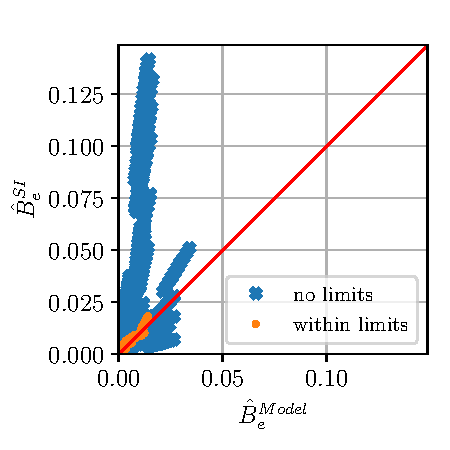
\includegraphics[width=\textwidth]{kappa/images/si_model_within.pdf}
        %\vspace{-0.5cm}
        \caption{The simplified Ikeda's method within and outside its limits.}
        \label{fig:si_model_within}
    \end{subfigure}
    \hfill
    \begin{subfigure}[b]{0.45\textwidth}
        \centering
        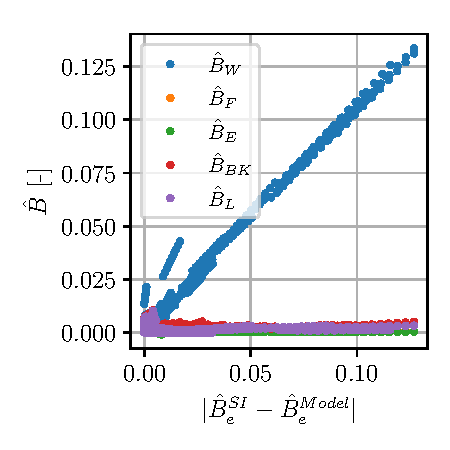
\includegraphics[width=\textwidth]{kappa/images/component_residual.pdf}
        \vspace{-0.2cm}
        \caption{Residuals vs. components.}
        \label{fig:component_residual}
        \vspace{0.3cm}
    \end{subfigure}
    \hfill
    \begin{subfigure}[b]{0.45\textwidth}
        \centering
        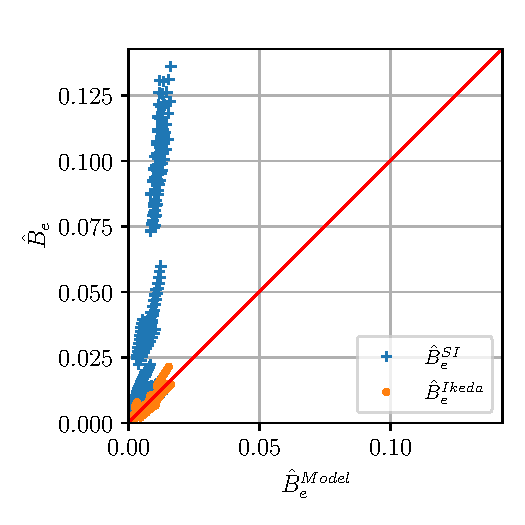
\includegraphics[width=\textwidth]{kappa/images/si_ikeda_model.pdf}
        \caption{Comparison of simplified and original Ikeda's method and model tests.}
        \label{fig:si_ikeda_model}
    \end{subfigure}

    \caption{Prediction error plots.}
\end{figure}

\begin{table}[H]
    \centering
    \caption{Validation of SI within and outside limits}
   \begin{tabular}{lrr}
\toprule
{} &  $R^2$ &  Number of points \\
\midrule
SI no limits     & -46.35 &              1470 \\
SI within limits &   0.83 &               120 \\
\bottomrule
\end{tabular}

    \label{tab:si_validation}
\end{table}
    
\noindent The largest contribution to the error in the predictions comes from the wave damping $B_W$, as seen in \autoref{fig:component_residual}. A comparison of the simplified Ikeda's method and the original Ikeda's method was carried out in Paper \ref{pap:rolldamping}; the comparison was used to determine whether the observed deviations are the result of extrapolation or inherent to the original method. In Ikeda's method, more extensive knowledge of the ship hull geometry is needed in order for $B_W$ to be calculated with a strip method and $B_E$ to be calculated with sectional Lewis coefficients. It was possible to collect the required hull inputs for 15 ships in the database. These ships were used in 50 of the reference roll decay tests; all but one of the tests exceed the limits. Ikeda's method has much more agreement for these exceeding model tests according to \autoref{fig:si_ikeda_model} and the calculated $R^2$ in Table \ref{tab:si_ikeda_validation}.


\begin{table}[H]
    \centering
    \caption{Validation of SI and Ikeda.}
   \begin{tabular}{lrr}
\toprule
{} &   $R^2$ &  Number of points \\
\midrule
Ikeda        &    0.84 &               500 \\
SI no limits & -127.95 &               500 \\
\bottomrule
\end{tabular}

    \label{tab:si_ikeda_validation}
\end{table}
    
\subsection{Generic roll damping model}
\label{sec:genericrolldampingmodel}
A serial grey-box model for ship roll damping (see \autoref{fig:greyrolldamping}) is also developed in Paper \ref{pap:rolldamping}. 
This is expanding the system identification by not only focusing on one ship, but all modern ships. 
The simplified Ikeda's method \cite{kawahara_simple_2011} is used as the white-box model, which is combined with the following black-box correction model.

\begin{figure}[H]
    
    \centering
    \begin{tikzpicture}[node distance=2cm]
    \node (white-box) [white-box] {\footnotesize Simplified Ikeda};
    \node (B_BK) [io, right of=white-box, xshift=0.90cm, yshift=1.5cm] {\footnotesize $\hat{B_{BK}}$};
    \node (B_E) [io, right of=white-box, xshift=0.75cm, yshift=0.75cm] {\footnotesize $\hat{B_{E}}$};
    \node (B_F) [io, right of=white-box, xshift=0.75cm, yshift=0cm] {\footnotesize $\hat{B_{F}}$};
    \node (B_L) [io, right of=white-box, xshift=0.75cm, yshift=-0.75cm] {\footnotesize $\hat{B_{L}}$};
    \node (B_W) [io, right of=white-box, xshift=0.75cm, yshift=-1.5cm] {\footnotesize $\hat{B_{W}}$};
    
    
    \node (black-box) [black-box, right of=B_F, xshift=0.75cm] {\footnotesize Black-box};
    \draw [arrow] (white-box) -- (B_BK);
    \draw [arrow] (white-box) -- (B_E);
    \draw [arrow] (white-box) -- (B_F);
    \draw [arrow] (white-box) -- (B_L);
    \draw [arrow] (white-box) -- (B_W);
    
    \draw [arrow] (B_BK) -- (black-box);
    \draw [arrow] (B_E)  -- (black-box);
    \draw [arrow] (B_F)  -- (black-box);
    \draw [arrow] (B_L)  -- (black-box);
    \draw [arrow] (B_W)  -- (black-box);
    
    
    \node (B) [io, right of=black-box, xshift=0.75cm, yshift=0cm] {\footnotesize $B$};
    \draw [arrow] (black-box)  -- (B);
    
    \end{tikzpicture}
    \caption{Grey-box model to predict roll damping.}
    \label{fig:greyrolldamping}
\end{figure}

\noindent The roll damping data set, obtained from the roll motion investigation, is intended to train the black-box component of the grey-box model. The black-box correction model of the output components from the simplified Ikeda's method is displayed in (\autoref{eq:polynom_correction}),
\begin{equation} \label{eq:polynom_correction}
\hat{B_{e}} = 1.106 \hat{B_{BK}} - 0.9124 \hat{B_{E}} + 4.282 \hat{B_{F}} + 0.7457 \hat{B_{L}} + 0.1844 \hat{B_{W}} + 0.004999 \phi_{a} - 0.0005097
\end{equation}


\noindent Major corrections to the skin friction damping $\hat{B_F}$ and wave damping $\hat{B_W}$ are included in this expression. The corrections are included because the simplified Ikeda's method is not very accurate for this dataset; most of the ships in the dataset exceeded the limits of the method. A pure black-box model is also developed in Paper \ref{pap:rolldamping} (see \autoref{eq:polynom_complex}),
\begin{equation} \label{eq:polynom_complex}
\begin{aligned} 
 \hat{B_{e}} = - 0.02578 A_{0} V - 0.02705 BK_{B} V + \\ 
 0.008993 BK_{L} V - 0.03191 C_{b} V - 0.2028 OG V + \\ 
 0.003472 V^{2} + \\ 
 0.004234 V \hat{\omega_{0}} - 0.002591 V \phi_{a} - 0.008384 V beam + \\ 
 0.05048 V + \\ 
 0.007814 \hat{\omega_{0}}^{2} + \\ 
 0.03882 \hat{\omega_{0}} \phi_{a} - 0.001069 \\ 
 \end{aligned}
\end{equation}

\noindent where non-dimensional frequency $\hat{\omega_0}$ is calculated with \autoref{eq:omega0_hat_equation} \cite{himeno_prediction_1981},
\begin{equation} \label{eq:omega0_hat_equation}
\omega_{hat} = \frac{\sqrt{2} \omega_{0} \sqrt{\frac{beam}{g}}}{2}
\end{equation}

Over-fitting data is a concern when constructing a regression model from a data set. Including too many parameters or allowing the order of the model to be too high would provide a very accurate representation of the present roll damping data. However, such a representation would be accompanied by major extrapolation errors when the model is used for other data. The generalization of the model can be assessed with a hold-out evaluation by using K-fold cross validation \cite{mosteller_handbook_1968} (\autoref{fig:k-fold}).\begin{figure}[h]
    \centering
    
    \begin{tikzpicture}
      \matrix (M) [matrix of nodes,
          nodes={minimum height = 7mm, minimum width = 1.2cm, outer sep=0, anchor=center,   draw},
          column 1/.style={nodes={draw=none}, minimum width = 4cm},
          row sep=1mm, column sep=-\pgflinewidth, nodes in empty cells,
          e/.style={fill=yellow!30}
        ]
        {
          Experiment 1 & & & & & |[e]| \\
          Experiment 2 & & & & |[e]| & \\
          Experiment 3 & & & |[e]| & & \\
          Experiment 4 & & |[e]| & & & \\
          Experiment 5 & |[e]| & & & & \\
        };
        \draw (M-1-2.north west) ++(0,2mm) coordinate (LT) edge[|<->|, >= latex]     node[above]{Total number of datasets} (LT-|M-1-6.north east);
        
        \node (training)[rectangle,
            draw,
            anchor=west,
            text = black,
            minimum width=2cm,
            fill = white] at (4.7,0.5) {Training};
            
        \node (validation)[rectangle,
            draw,
            anchor=west,
            text = black,
            minimum width=2cm,
            fill = yellow!30, below of=training]{Validation};
        
    \end{tikzpicture}
    
    \caption{K-fold cross validation}
    \label{fig:k-fold}
\end{figure} The data has been divided into five smaller sets (folds). Four of the folds are used to train the model, and the fifth fold is used for testing (validation). Validation consists of calculating the coefficient of determination $R^2$ for the fitted model. Validation is completed for all five possible train-test combinations. 
The folds are randomly constructed with the restriction that all data for a particular ship must be in the same fold. Five folds are randomly generated 20 times, which gives 100 values of $R^2$ from the train-test-procedure for each model. The mean values and standard deviation of these 100 values of $R^2$ are displayed in Table \ref{tab:crossvalidation}. The mean and standard deviation of $R^2$ simplified Ikeda's method in this table were calculated directly instead of using cross validation because they do not rely on the SSPA data.

\begin{table}[H]
    \centering
    \caption{Statistics from cross validations with all models.}
   \begin{tabular}{lrr}
\toprule
{} &  $E[R^2]$ &  $std(R^2)$ \\
model                      &           &             \\
\midrule
Simplified Ikeda corrected &      0.75 &        0.16 \\
New regression             &      0.77 &        0.09 \\
\bottomrule
\end{tabular}

    \label{tab:crossvalidation}
\end{table}
    
\clearpage